\documentclass[12pt]{article}

\usepackage{times}          % Times New Roman font
\usepackage{setspace}       % Double spacing
\usepackage[letterpaper, margin=1in]{geometry}  % 8.5x11, 1" margins
\usepackage[utf8]{inputenc}
\usepackage{amsmath}
\usepackage{amsfonts}
\usepackage{amssymb}
\usepackage{cleveref}
%\usepackage[font=small,labelfont=bf]{caption}
\usepackage{float}
\usepackage{graphicx}
\graphicspath{{""}{fig/}} %Figure path
\usepackage{natbib}
\setcitestyle{authoryear,open={(},close={)}} %Citation-related commands
\setcitestyle{aysep={}}
\setcitestyle{citesep={,}}
\usepackage{url}
\usepackage{tabularx}
\usepackage{lipsum}
\usepackage{verbatim}
\usepackage{tcolorbox}
\usepackage{bm}
\usepackage{xr}
\usepackage{lineno}
\setlength{\parskip}{0.5\baselineskip}

%\captionsetup{justification=raggedright, singlelinecheck=false}%, font=doublespacing}

\DeclareMathOperator\erf{erf}
\newcommand{\mat}[1]{\bm{#1}}

% Page layout
\topmargin -1.0cm
\oddsidemargin 0.5cm
\evensidemargin 0.5cm
\textwidth 16cm
\textheight 23cm

\tolerance=1
\emergencystretch=\maxdimen
\hyphenpenalty=10000
\clubpenalty=10000
\widowpenalty=10000
\hbadness=10000
\raggedright

%External references (SI)
\makeatletter
\newcommand{\ud}{\text{d}}
\let\originalleft\left
\let\originalright\right
\renewcommand{\left}{\mathopen{}\mathclose\bgroup\originalleft}
\renewcommand{\right}{\aftergroup\egroup\originalright}
\newcommand*{\addFileDependency}[1]{% argument=file name and extension
\typeout{(#1)}% latexmk will find this if $recorder=0
% however, in that case, it will ignore #1 if it is a .aux or
% .pdf file etc and it exists! If it doesn't exist, it will appear
% in the list of dependents regardless)
%
% Write the following if you want it to appear in \listfiles
% --- although not really necessary and latexmk doesn't use this
%
\@addtofilelist{#1}
%
% latexmk will find this message if #1 doesn't exist (yet)
\IfFileExists{#1}{}{\typeout{No file #1.}}
}\makeatother

\newcommand*{\myexternaldocument}[1]{%
\externaldocument{#1}%
\addFileDependency{#1.tex}%
\addFileDependency{#1.aux}%
}

\graphicspath{{../figures/}}
\myexternaldocument{supplementary}

\title{\vspace{-1.5cm}{Eco-evolutionary dynamics hinder recovery in harvested populations}}
%Competitive traps from eco-evolutionary feedbacks hinder recovery in harvested fish populations
% Eco-evolutionary trait changes hinders recovery after population collaps



\author{Mikael Ohlsson\textsuperscript{1},
György Barabás\textsuperscript{1,2},
Max Lindmark\textsuperscript{3},\\
Michele Casini\textsuperscript{3,4},
Viktor Thunell\textsuperscript{3},
Valerio Bartolino\textsuperscript{3},
Mattias Sköld\textsuperscript{3},
Anna Eklöf\textsuperscript{1*}}

\date{}

\linenumbers


\begin{document}

\maketitle
    $^1$ Department of Physics, Chemistry and Biology, Linköping University, 581 83 Linköping, Sweden\\[1.2ex]%
    $^2$  HUN-REN Centre for Ecological Research, Institute of Evolution, Budapest, Hungary\\[1.2ex]
    $^3$ Department of Aquatic Resources, Institute of Marine Research, Swedish University of Agricultural Sciences,  Turistgatan 5, 453 30 Lysekil, Sweden\\[1.2ex]%
    $^4$ Department of Biological, Geological and Environmental Sciences (BiGeA), University of Bologna, Via Selmi 3, 40126 Bologna, Italy\\[1.2ex]%
    \textsuperscript{*}Corresponding author. E-mail: anna.eklof@liu.se\\[2.0ex]%

\paragraph{Author contributions} M.O., G.B., and A.E. designed the study. M.O. and G.B. wrote the code for the eco-evolutionary model. M.L. and M.C. constructed the model for predicting biomass densities. M.O. performed the simulations and analysis. M.O., G.B., and A.E. wrote the paper. All authors made significant contributions to the final version of the manuscript.

\paragraph{Keywords}
Alternative stable states, cod, competition, Baltic Sea, body size, eco-evolutionary dynamics, flounder, overfishing, population recovery



\paragraph{Open Research statement:} Data and computer code for implementing the model and replicating results is available at \url{https://github.com/MikaelOhlsson/CodFleEcoEvo}. They will be deposited at zenodo.org, pending acceptance of the manuscript.

\clearpage
\doublespacing

\begin{abstract}
\noindent Intense harvesting and environmental shifts can trigger population collapse that fails to rebound even after stressors are removed. Yet, why recovery fails so frequently remains elusive. Here we start from the observation that stressors are often accompanied by considerable selection pressure (for example, fishing generally targets larger individuals), and propose that the ensuing trait evolution can generate competitive traps: by shifting a focal species into a competitor's ecological niche, externally imposed trait change intensifies interspecific competition and locks the focal population in an altered state independently of the original stressor. Using an eco-evolutionary model that couples population dynamics with trait evolution, we show that this mechanism produces alternative stable states separated by a tipping point defined by the competitor's trait distribution, such that recovery requires escaping not just the original pressure but the competitive feedback it has created. We illustrate this with Atlantic cod (\textit{Gadus morhua)} in the Baltic Sea, where fishing-driven reductions in body size have shifted cod into dietary overlap with the flounder (\textit{Platichthys flesus}) population, precisely the competitive reorganization our model predicts. These findings suggest that eco-evolutionary feedbacks may represent an underappreciated mechanism maintaining unfavorable population states, and that management focused solely on reducing harvest pressure risks missing the evolutionary legacies that disturbance leaves behind.
\end{abstract}

\clearpage

\section*{Introduction}
Severe ecological transitions occur across a wide range of ecosystems, including collapses of exploited populations in marine environments \citep{Hutchings2004, Neubauer2013}, vegetation shifts in drylands \citep{kefi2007spatial, scheffer2001catastrophic}, and insect-driven transitions in plant communities  \citep{agrawal2012insect}. Although such transitions are often triggered by external drivers, e.g. harvesting, grazing or environmental change, many systems fail to return to their previous state even after these drivers are reduced or even removed \citep{Hutchings2004}. One explanation is that disturbances shift key functional trait distributions within populations, thereby reshaping species interactions within communities \citep{kelley2018habitat}. % TO DISCUSSION: When such trait distributions shift, the resulting changes in species interactions may generate eco-evolutionary feedbacks in which ecological dynamics and trait evolution reinforce each other \citep{hart2019effects, fussmann2007eco} potentially hindering recovery.


Body size provides a highly relevant example of such a trait, as it governs metabolic demands, trophic position, and dietary preferences, thereby shaping both competitive and predator-prey interactions \citep{Ahti2020, Beverton2012}. Because body size is heritable, sustained directional pressures can drive evolutionary changes in size distributions within populations \citep{Nielsen2014, Kuparinen2017}. Crucially, these evolutionary changes are not ecologically neutral; a reduction in body size can alter dietary niche, competitive relationships, and vulnerability to predation, potentially generating eco-evolutionary feedbacks that impede recovery \citep{Edeline2021}.


Such eco-evolutionary feedbacks may be particularly pronounced in systems subject to multiple simultaneous pressures \citep{cote2016interactions, crain2008interactive, cuenca2021evolutionary}. In marine fish populations, for example, decades of environmental change and anthropogenic pressures have driven population collapses across many taxa  \citep{Hutchings2004, Neubauer2013}. Although recovery following reduced pressure has been documented in some marine fish stocks \citep{Hilborn2009, Duarte2020}, many populations remain at low abundance or continue to decline despite such reductions \citep{Kuparinen2014, Neuenhoff2019}. The slow or absent recovery for these populations is typically attributed to Allee effects, where a smaller population size interferes with recovery \citep{Kuparinen2014}. However, such explanations are generally only partially sufficient, as with time, populations are expected to recover after fishing stops unless other factors interact \citep{Neuenhoff2019}.


The collapse of Eastern Baltic cod (\textit{Gadus morhua}) provides a useful case for examining these dynamics. The Baltic Sea is a semi-enclosed basin that has undergone extensive environmental change, including a significant expansion of hypoxic and anoxic zones \citep{Carstensen2014}, which directly impair fish growth and reduce available habitat \citep{Casini2016, Bartolino2017, Orio2019, Orio2020, Lindmark2023}. Simultaneously, intense size-selective fishing has contributed to the collapse of the cod population, characterized by sharp declines in abundance, body size, and geographic range \citep{Orio2020, ICES2022}. As cod contracted their range toward better-oxygenated areas, spatial overlap with the flounder species complex (\textit{Platichthys flesus} and \textit{P. solemdali}; hereafter flounder) increased. Flounder has expanded in both abundance \citep{ICES_18645_2025, ICES2022} and distribution \citep{Orio2020} over the same period, potentially intensifying competition for shared benthic prey---particularly the isopod \textit{Saduria entomon} \citep{Haase2020}. Coinciding with the decline of \textit{Saduria} in cod diets \citep{Haase2020}, small cod have shifted from benthic invertebrates toward more piscivorous diets \citep{ICES2015, Haase2020}. Despite the recent cessation of cod fishing \citep{ICES2022}, there are no signs of recovery in abundance or condition \citep{ICES2022}.

Here we develop a general an eco-evolutionary model that tracks species' trait changes under both environmental and anthropogenic effects, while simultaneously accounting for changes in interspecific interactions. The model allows competitive interactions to change dynamically as trait distributions evolve, and is sufficiently flexible to incorporate a wide range of processes thought to be relevant in any given ecological situation---such as fishing pressure and hypoxia for the Baltic Sea cod-flounder system. We then argue that the proposed eco-evolutionary mechanism not only provides a robust theoretical explanation for the observed lack of recovery in cod abundance and body size, but is also consistent with long-term observational data from the Baltic Sea. This case study is therefore a good candidate for an empirical system where competitive relationships lock populations into alternative trait states, providing a potential explanation for the lack of recovery for Baltic cod and highlighting a general mechanism by which eco-evolutionary feedbacks can undermine ecological resilience.



\section*{Methods}

\subsection*{Eco-evolutionary dynamics}

Our eco-evolutionary model tracks the population densities and trait (body size, denoted by $z$) distributions of two competing consumer species through time: a focal species subject to size-selective harvesting, and a competitor species whose size distribution is assumed not to evolve. We assume that the the body size of an individual and the average size of its resources are sufficiently tightly correlated that $z$ need not refer to the actual body size, but instead to the mean body size of its prey \citep{Rossberg2013, Schneideretal2016}. Thus, we define $z = \log(B/B_0)$, where $B$ is the average resource size (assumed to be in a quasi-one-to-one relationship with the modeled consumer individual's size) and $B_0$ is a reference size which can be chosen without loss of generality. Here we set $B_0$ to be the mean prey size of the competitor species, so that $z = 0$ corresponds to the point at which the mean prey sizes of the two competing consumers coincide.

The assumption that the competitor body sizes do not evolve means that $B_0$ is constant. To describe the interactions between the two species, we assume that they compete for shared resources. In general, dietary overlap between competing consumers may be incomplete. To account for this, we model resource consumption in a potentially high-dimensional trait space, the first dimension of which is the body size $z$. Additional traits---such as habitat preference, locomotion, or foraging behaviour---contribute to resource utilization but are not under evolutionary influence. Since we assume that the primary driver of trait change in the focal species primarily selects for size, we ignore selection on the other traits.

In case body size variation is influenced by many additive loci with small effects, the infinitesimal model of quantitative genetics \citep{Barton2017} is suitable to model the eco-evolutionary dynamics of the population densities $N_i$ and mean body sizes $\mu_i$, where $i$ indexes the competing consumer species. The trait distributions $p_i(z)$ are then normal, and the genetic variances $\sigma_i^2$ are assumed to be constant and to not change in response to selection (for the evolution of trait variances and their eco-evolutionary consequences, see \citealp{TaperCase1985, MullonLehmann2019, Barabasetal2022}, and \citealp{Wickmanetal2023}). Consequently, the heritabilities $h_i^2$ (ratio of genetic to total phenotypic variance) are also constant. With these assumptions, and given an expression for the per capita growth rates $r(z)$ of individuals with body size $z$, the following general equations govern the dynamics of the population densities and body sizes:
\begin{align}
  \label{eq-n-general}
  \frac{\ud N_i}{\ud t}
  &= N_i \int r(z) p_i(z) \,\ud z \\
  \label{eq-mu-general}
  \frac{\ud \mu_i}{\ud t}
  &= h_i^2
  \int (z - \mu_i) r(z) p_i(z) \,\ud z
\end{align}
where the integration goes across the entire trait space \citep{    Slatkin1979, Slatkin1980, TaperCase1985, Schreiberetal2011, Vasseuretal2011, Barabas2016, MullonLehmann2019, Pastore2021, Barabasetal2022, baruah2025when}.

Applying this general framework to the Baltic Sea cod-flounder system, the per capita growth rates are determined by four distinct processes: (1) growth due to consumption of resources (this implicitly contains competition across phenotypes when their resources are shared), (2) natural mortality, (3) mortality due to size-dependent fishing pressure, and (4) mortality from oxygen-deprived regions which affect bigger individuals more due to different food-seeking behavior. Expressing these processes mathematically, writing the resulting growth rates into the general set of equations \eqref{eq-n-general}-\eqref{eq-mu-general}, and performing all integrations (Supplement S1-S2), we get:
\begin{equation}
  \label{eq-n}
  \frac{\ud N_i}{\ud t}
  = N_i \Bigg[ \underbrace{\frac{\varrho}{\theta^2}
  \left(\theta^2 - (z^*-\mu_i)^2 - \sigma_i^2 \right)}_{\text{intrinsic growth}}
  - \underbrace{\eta Q\left(\frac{\mu_i-\varphi}
  {\sqrt{2\sigma_i^2+\tau^2}}\right)}_{\text{fishing mortality}}
  - \underbrace{\kappa Q \left(\frac{\mu_i-\zeta}
  {\sqrt{2\sigma_i^2+\nu^2}}\right)}_{\text{hypoxic mortality}}
  - \underbrace{\sum_j \alpha_{ij} N_j}_{\text{resource comp.}} \Bigg]
\end{equation}
\begin{equation}
  \label{eq-mu}
  \begin{split}
  \frac{\ud \mu_i}{\ud t}
  &= h_i^2 \Bigg[
  \underbrace{\frac{2\varrho\sigma_i^2}{\theta^2}\left(z^*-\mu_i\right)}_{\text{selection from growth}} -
  \underbrace{\frac{\eta\sigma_i^2}{\sqrt{\pi(2\sigma_i^2+\tau^2)}}
  \exp\left( -\frac{(\mu_i-\varphi)^2}{2\sigma_i^2+\tau^2}\right)}_{\text{selection from fishing}}
  \\ & \qquad\qquad\quad -
  \underbrace{\frac{\kappa\sigma_i^2}{\sqrt{\pi(2\sigma_i^2+\nu^2)}}
  \exp\left( -\frac{(\mu_i-\zeta)^2}{2\sigma_i^2+\nu^2} \right)}_{\text{selection from hypoxia}}
  + \underbrace{\sum_j \frac{(\mu_i - \mu_j) \sigma_i^2}{\sigma_i^2 + \sigma_j^2 + \omega^2} \alpha_{ij} N_j}_{\text{selection from competition}} \Bigg]
  \end{split}
\end{equation}
Here $\varrho$ is the maximum intrinsic growth rate (achievable in the absence of any competition and when $\mu_i$ equals the optimal body size $z^*$), and $\theta$ is the width of the body size region where positive intrinsic growth is possible. To interpret the parameters related to harvesting, we first observe that size-dependent harvesting such as fishing often saturates for large body sizes \citep{Brinkhof2020}. We thus describe mortality from harvesting as a sigmoid function $Q(z) = (\erf(z) + 1)/2$ of body size, where $\erf(z)$ is the error function. Then, the parameter $\eta$ is the harvesting effort (maximum harvesting rate for large $z$), $\varphi$ is the size where mortality from harvesting reaches half its maximum, and $\tau$ is the width of the transition from low to high values of the sigmoid curve. Similarly, reduction in growth caused by an additional external pressures, here exemplified with hypoxia, is also described by a sigmoid curve, with smaller phenotypes affected less than larger phenotypes. Thus, $\kappa$ is the maximum reduction in growth caused by hypoxia, $\zeta$ is the size at which hypoxia starts having a strong effect, and $\nu$ is the abruptness of the transition.

Finally, $\alpha_{ij}$ is the competitive effect exerted by species $j$ on species $i$. This is derived from an explicit consumer-resource interaction model (Supplement S1-S2), and reads:
\begin{equation}
  \label{eq-alpha}
  \alpha_{ij}
  = \frac{\alpha_0}
  {\sqrt{2\pi(\sigma_i^2 + \sigma_j^2 + \omega^2)}}
  \exp \left( -\frac{(\mu_i - \mu_j)^2}
  {2(\sigma_i^2 + \sigma_j^2 + \omega^2)} \right)
  \times
  \begin{cases}
    \begin{array}{ll}
      1 & \text{if~} i = j \\
      \alpha_I & \text{otherwise}
    \end{array}
  \end{cases}
\end{equation}
This is a Gaussian function of the difference in mean body sizes $|\mu_i - \mu_j|$, and so species experience maximal competition when their mean traits are equal, with competition declining as the trait difference increases. The parameter $\omega^2$ is the variance of this Gaussian before it is integrated across the phenotype distributions of the species (after integration, it becomes $\sigma_i^2 + \sigma_j^2 + \omega^2$, as seen in Eq.~\ref{eq-alpha}). $\alpha_0$ simply scales the coefficients to give them correct units. As mentioned before, species may differ in traits other than body size. In case overlap in these other, non-evolving traits is only partial, resource competition is somewhat alleviated. The degree to which this happens is measured by $0 < \alpha_I \le 1$, with $\alpha_I = 1$ corresponding to full overlap (i.e., species truly only differ in body size and nothing else), and lower values to partial overlap (Supplement S2).

One important simplification to the model is to assume that the competitor population density is constant, being at some fixed equilibrium value. Let the species index $i$ be either $C$ (cod; the focal species) or $F$ (flounder; the competitor). We then set $N_F$ constant. This allows one to reason about body size evolution much more simply, because Eq.~\ref{eq-mu} for the focal species decouples from Eq.~\ref{eq-n}. Further, $\mu_F = 0$ is a constant parameter, since we assumed that body size of the competitor does not evolve ($h_F^2 = 0$). That is, Eq.~\ref{eq-mu} for the focal species reduces to the one-dimensional dynamical system $\ud \mu / \ud t = g(\mu)$, where $\mu = \mu_C$ is a simplified notation for the focal species' mean size and $g(\mu)$ is the right hand side of Eq.~\ref{eq-mu} after fixing $N_F = \text{const.}$ and $\mu_F = 0$. The curves in the right column of Fig.~\ref{fig:sizegrid} are plotted using this function. It turns out that the predicted body size dynamics from this decoupled and simplified equation are qualitatively identical to those from the full model (Supplement S2).


\subsection*{Empirical comparison}

To illustrate the model with an empirical case study, we apply it to cod and flounder populations in the Baltic Sea. We use survey data for both species to estimate annual indices of relative biomass, mean length-at-age, and dietary overlap between size classes of cod and flounder. We then compare these qualitatively with model expectations to support the model's conclusions.

\subsubsection*{Data}

We used data from the Baltic International Trawl Survey (BITS) to evaluate relative biomasses and diets of cod and flounder in the southern Baltic Sea. BITS is a bi-annual bottom trawl survey, conducted during quarters one and four. Data on catch per unit effort can be downloaded from the ICES DATRAS database (\url{https://datras.ices.dk/}). We standardized these data for differences in gear following \citep{Orio2017, Lindmark2023}, to acquire survey catches in density per area (kg/km\textsuperscript{2}). Cod and flounder body lengths for 1978–2023 were also extracted from the DATRAS database, from which we calculated the annual mean and 95th percentile of length.

The stomach content data for cod and flounder were compiled from different sources. The majority of the cod stomach data have been collated in EU funded projects \citep{huwerStudyStomachContent2014, jacobsenStudyStomachContent2023} and are available at the International Council for the Exploration of the Sea (ICES) stomach content database (\url{https://www.ices.dk/data/data-portals/Pages/Stomach-content.aspx}). In addition, we used recent cod stomach data collated in \citep{lindmarkWeakEffectsLocal2025a}. Flounder stomach data are from \citep{lindmark2025quantifying}. This compiled data set comprised cod stomach data between 1963 and 2023 and flounder stomach data between 2015 and 2022. For both species, data collected from 1993 and onwards were mainly collected on the bi-annual Baltic International Trawl Survey (BITS) conducted in the first and fourth quarter of the year, but also from other cruises conducted in other times of the year (see \citep{huwerStudyStomachContent2014}, \citep{jacobsenStudyStomachContent2023}, and \citep{lindmark2025quantifying, lindmarkWeakEffectsLocal2025a} for a detailed description of the data sources). The stomach samples included data for individuals larger than 6 cm and were separated into quarters one and four. Whenever possible, one flounder and one cod stomach were collected for each cm class of fish length and trawl haul. Prey items were grouped into 15 taxonomic groups based on \citep{Haase2020}.

\subsubsection*{Biomass model}
We fit the survey catch data with a geostatistical generalized linear mixed-effects model, using a Tweedie distribution \citep{Tweedie1984, Shono2008, sdmTMB} and a log-link function, due to the presence of zeros and continuous densities. For details about the biomass model, we refer to Supplement~S3 and \citep{Lindmark2023}. We used this model to predict the biomass density of cod and flounder over a regular grid of 4 $\times$ 4 km squares with covariates to calculate annual indices of relative biomass based on a random-field model \citep{Shelton2014, Thorson2015} over the spatial domain. While the model was fit to data from years 1993–2020 in ICES subdivisions 24--28, we only make predictions for subdivisions 25--28 to match where we have the most diet data (Supplementary Fig.~S3), while excluding subdivision 24 where mixing with the western cod population occurs more frequently.

\subsubsection*{Diet overlap}
We used the stomach content data to calculate the dietary distance, and thus possible interspecific competition, between cod and flounder. We aggregated cod and flounder data into arbitrary length classes (Cod $<$ 10 cm, 10-15 cm, 15-20 cm, 20-25 cm, 25-30 cm, 30-40 cm, 40-50 cm and $>$ 50 cm, flounder $<$ 20 cm, 20--30 cm, and $>$ 30 cm). Stomach content weight was used for calculating dietary proportions and dietary distances. For each individual sample, prey proportions based on the respective prey species weights were calculated. These were then used to obtain the average dietary proportions for the respective time periods and size classes. The proportions were then used to calculate the dietary distances using the Horn--Morisita index with the \texttt{abdiv} package \citep[version 0.2.0,][]{Bittinger2020} in R \citep{R}, where the dissimilarity between two vectors $x$ and $y$ consisting of, in our case, the dietary proportion elements $i$ is described as:
\begin{equation}
  \label{eq-mori}
  d(x,y)
  = 1 - \frac{2 \sum_i x_i y_i}{\left( \dfrac{\sum_j x_j^2 }{\mat{N}_x^2} + \dfrac{\sum_k y_k^2 }{\mat{N}_y^2} \right) \mat{N}_x\mat{N}_y}
\end{equation}
where $\mat{N}_x = \sum_i x_i$. The resulting distance index has a value of 0 if the diets are identical and 1 if the diets have nothing in common.


\section*{Results}

Our eco-evolutionary model shows that when the focal species' body sizes are initially large and harvesting is absent to moderate, the opposing selective pressures from the environment and from resource competition create an equilibrium for the focal species' size at point $c$ in Fig.~\ref{fig:sizegrid}AB. The rate of change in body size $\mu$ has one unstable equilibrium $b$ and two stable equilibria at $a$ and $c$ (Fig.~\ref{fig:sizegrid}B). The unstable equilibrium at point $b$ is centered close to the competitor's mean size $\mu_{F}$, with environmental factors causing a slight offset. The presence of the competitor keeps the focal species' size from crossing the unstable point, and so the alternative stable equilibrium at $a$ (where the focal species body sizes are much smaller) is unattainable.

However, sufficiently intensive harvesting will eventually overcome the competitive pressure (Fig.~\ref{fig:sizegrid}D), forcing the focal species' body size distribution to go below that of its competitor and cross into the alternative, smaller-sized stable state. Now, with the focal species' size distribution in panel E, resource competition pushes the focal species towards smaller body sizes, keeping it locked in its smaller state even after fully relieving the harvesting pressure (Fig.~\ref{fig:sizegrid}F, point $a$). The system has thus undergone a critical transition and is now trapped at the undesirable equilibrium point corresponding to small body sizes.

\subsection*{Case study: cod and flounder in the Baltic Sea}

We now apply our modelling framework to data from the Baltic Sea cod and flounder populations. While the cod population has steadily declined since the early 1990s, flounder has increased in recent years (Fig.~\ref{fig:biomasslength}A).

% Fig 2 was here

Simultaneously, both cod and flounder have decreased in body size, although this decrease was more extreme for cod (Fig.~\ref{fig:biomasslength}B). Large individuals in particular have practically disappeared, with the 95th percentile of length decreasing from 70 cm in 1993 to 40 cm in 2023. In addition, there has been a clear shift in cod diet from a largely benthic to a piscivorous diet (Fig.~\ref{fig:diet_prop}). This dietary shift has propagated through all but the smallest size classes of cod.

% Fig 3 was here

Historical data on flounder stomach content from the Baltic Sea is not available, limiting dietary comparisons to the flounder diet to years 2015--2020. However, given the relatively limited body size change of flounder (Fig.~\ref{fig:biomasslength}B), and flounder being an obligate benthic feeder, we can assume the flounder diet to be constant, and compare the historical cod dietary data with the current flounder diet (Fig.~\ref{fig:diet_dist}). Historically, mid-range to larger cod sizes had a more similar diet to flounder. However, in recent years, the larger-sized cod diet has diverged, explained by their change towards a piscivorous diet. In contrast, smaller cod (10–30 cm) now display greater overlap with flounder in their diet.

% Fig 4 was here

\section*{Discussion}

Our results demonstrate that fishing-driven reductions in body size can push cod into a trait range where competitive interactions with flounder are intensified, and that this competitive pressure alone is sufficient to maintain cod in a small-bodied state independently of fishing mortality. This eco-evolutionary lock-in offers a mechanistic explanation for the persistent failure of Baltic cod to recover despite decades of reduced harvest pressure \citep{Koster2017, Mion2021, ICES2022}, and suggests that the system may have shifted into a self-reinforcing state from which recovery through reduced fishing alone is unlikely to be sufficient.

The underlying mechanism --an external pressure shifting a focal species into a trait range that intensifies competition with a sympatric competitor, which in turn maintains the evolved state -- is not unique to harvested fish populations. While the individual components of this mechanism are well established, the complete causal chain has not previously been demonstrated. External pressures such as environmental change are known to shape trait evolution with cascading effects on species interactions \citep{ehrlich2025role}. These evolutionary responses can restructure competitive hierarchies and reinforce altered community states \citep{hart2019effects}, even when the evolving traits are not directly linked to resource competition \citep{mougi2007evolution}. While competition can in some cases drive trait divergence and reduced niche overlap \citep{clarke2017trait}, such divergence may also involve trade-offs that constrain species to particular regions of trait space. Moreover, historical competition can leave lasting evolutionary legacies that influence future dynamics and recovery potential \citep{govaert2021competition}. A related dynamic is observed in plant communities, where changes in insect herbivory rate have been shown to shift competitive traits in a focal species, enabling a competitor to expand and lock the focal plant into an altered competitive state \citep{agrawal2012insect}.

The Baltic Sea cod-flounder system provides a case where each component of this mechanism can be traced, and where the full causal chain connects external pressure, trait evolution, and competitive feedback. Cod diet differs strongly between size classes, whereas flounder is a specialized benthic feeder with a relatively narrow diet and limited ontogenetic dietary shift \citep{Haase2020}. Cod has also historically exhibited considerable individual variation in dietary preferences, suggesting a high degree of feeding adaptability \citep{Haase2020}. Flounder's dietary specialization, combined with the increase in flounder abundance, explains why cod rather than flounder is the species shifting its ecological niche under competitive pressure. As fishing selectively removes larger individuals and shifts the cod size distribution downward, flounder exerts stronger competitive pressure on a larger fraction of the cod population, an effect further amplified by increased spatial overlap between the species. Our model demonstrates this mechanism by identifying two alternative equilibria for cod body size: when cod maintain a sufficiently large mean body size, their ecological niche remains separated from flounder and the large-bodied state is self-reinforcing. When fishing pressure is intense enough to push cod below a size threshold, resource competition with flounder increases and the only stable equilibrium shifts to the small-bodied state. This unstable intermediate acts as a tipping point \citep{Dakos2022}: cod must surpass it to recover, but competitive pressure from flounder prevents this even after fishing is removed (Fig.~S2).

Empirical support for this competitive dynamic comes from observed dietary shifts in Baltic cod \citep{Kulatska2019, Haase2020, Neuenfeldt2020}. All but the smallest cod have shifted from a diet dominated by benthic invertebrates toward increasingly piscivorous feeding (Fig.~\ref{fig:diet_prop}). Although flounder diet data are only available from 2015 onwards, flounder's benthic specialization makes large dietary variation unlikely. Comparing present-day flounder diet with historical cod diet suggests that larger cod have shifted away from the benthic prey base they once shared with flounder, resulting in reduced dietary overlap (Fig.~\ref{fig:diet_dist}). Notably, cod have moved away from a historically Saduria-rich diet while flounder continue to rely heavily on Saduria---a prey known to be high in essential fatty acids and linked to improved cod body condition \citep{Lindmark2023, Rojbek2012}. The increased dietary overlap observed in smaller cod likely reflects shared consumption of other benthic invertebrates, consistent with a broader shift in benthic community composition \citep{Gogina2016}. Similar patterns of intensified competition with ecologically similar species following stock collapse have been observed in other cod populations \citep{Bundy2005, Walters2001}, suggesting the dynamic is not Baltic-specific. Taken together, these dietary shifts are consistent with competitive reorganization driven by increased flounder abundance rather than changes in prey availability alone. Hypoxia represents an additional synergizing factor, contracting the distributions of both species and thereby intensifying spatial overlap and competitive pressure \citep{Orio2019}, while also imposing disproportionate metabolic costs on larger cod \citep{Rubalcaba2020}, further reinforcing the size-selective pressure that fishing exerts.

Recovery from the small-bodied state is possible in our model when both fishing pressure and flounder competition are reduced, but if the size shift has a genetic basis, recovery may be slow. Natural selection generally favors larger body size through improved survival \citep{Olsen2011} and, critically, through hyper-allometric reproductive scaling: larger cod produce disproportionately more offspring than equivalent biomass distributed across smaller individuals \citep{Barneche2018}. A population depleted of large individuals therefore faces compounding disadvantages for recruitment and recovery that extend well beyond the direct effects of fishing. The genetic basis for observed size changes in Baltic cod is increasingly supported empirically. Declining growth rates in larger individuals \citep{Mion2021}, smaller body size at age \citep{ICES2022}, and earlier maturation \citep{Koster2017} together indicate that the size shift is not simply a demographic artifact of removing old large fish. A recent genomic study confirms this interpretation, finding that intensive fishing has left detectable signatures of directional selection across the cod genome \citep{han2025genomic}.

There are limitations to our modeling approach and its connection to empirical data. First, we focus on a single evolving trait, whereas in reality multiple traits may respond simultaneously and in different directions. Fishing can impose selection on both growth rate and body size, which are linked but not identical processes \citep{Rubalcaba2020}, and our model necessarily represents a simplification of this complexity. Second, we interpret the observed dietary data as reflecting a competitive reorganization that has already reached a new steady state, and we assume that dietary shifts in cod were driven largely by competition from flounder rather than independent changes in prey availability or spatial overlap \citep{Enberg2012}. Lastly, the empirical interpretation of our bistability result depends on the assumption that, in the absence of both fishing and flounder competition, cod would evolve toward the flounder size niche. If cod would instead evolve toward larger body sizes regardless of flounder, the observed correlation between flounder abundance and dietary distance would reflect processes outside our model rather than competitive dynamics.

The core mechanism of an external pressure shifting a species' trait into an alternative stable state is not unique to harvested fish populations. Beyond harvested systems, insect herbivory can also shift competitive traits in plant populations; \citet{agrawal2012insect} showed that altered herbivory reshaped the genetic structure of a focal plant population within three to four generations, thereby shifting the competitive balance between species. \cite{chaparro2021adaptive} used shallow lakes as a model ecosystem, investigating how trait evolution of a key species affects ecosystem states (turbid versus clear water) under environmental pressure. They showed that if evolutionary responses are constrained, such as limited genetic variation or interference from trade-offs with traits that mediate interspecific competition, the ecosystem can stay locked in the less desirable state.  The broader class of systems exhibiting transition irreversibility through biotic feedbacks includes dryland ecosystems, where the interplay between facilitation and competition can generate feedbacks that maintain altered community configurations and hinder recovery following environmental pressures \citep{kefi2008evolution, pichon2024interplay}.

More generally, our results are consistent with the growing recognition that eco-evolutionary feedbacks can shape ecosystem tipping points \citep{dakos2019ecosystem}, and that adaptation to a disturbed state can delay or prevent recovery even after the original stressor is removed \citep{chaparro2021adaptive}. Such responses can arise due to external pressures reshaping trait distributions and competitive interactions \citep{ehrlich2025role, hart2019effects}, reinforcing altered system states. Our results have implications for both the management of exploited populations and the design of restoration efforts. In particular, they suggest that the window for successful recovery may be time-limited. If eco-evolutionary feedbacks become established before intervention, the system may become locked in an altered state where reducing the primary stressor is insufficient. Early intervention, i.e. before trait distributions have shifted beyond a tipping point, may therefore be critical for preserving recovery potential. Identifying relevant competitors, understanding how trait shifts alter competitive interactions, and accounting for the resulting feedbacks may be as important for management as controlling the primary disturbance itself.


\subsection*{Conclusions}

We have shown that externally driven trait evolution and interspecific competition can interact to generate a competitive trap, in which a focal species is maintained in an altered state independently of the original pressure. In the Baltic Sea, this dynamic is mediated through eco-evolutionary feedbacks between fishing-induced body size reduction, resource overlap with flounder, and competitive interactions, offering a parsimonious explanation for why cod has failed to recover despite reduced harvest pressure. Body size is a key mediator of this process: because it governs both the direct targets of size-selective disturbance and the ecological interactions that respond to trait change, it links evolutionary and community-level dynamics in ways that purely demographic models do not capture. Recognizing competitive traps of this kind (identifying the competitor, characterizing the trait overlap, and locating the tipping point) may be as important for management as controlling the primary disturbance itself, both in the Baltic Sea and more widely.


% Notes - refs to add.
% The paper by \cite{clarke2017trait} shows that increasing competition can drive greater trait divergence (character displacement), and one could further hypothesize that such divergence, through trade-offs and specialization, may constrain species to particular regions of trait space, potentially reducing their competitive ability outside those niches.

% The paper by \cite{ehrlich2025role} shows that external pressures, such as environmental change or altered predation, play a key role in shaping trait evolution, which in turn can modify species interactions through feedbacks between trophic levels.

% \cite{hart2019effects} highlights that evolutionary changes in response to interspecific competition can alter competitive hierarchies, sometimes disadvantaging one species. Although the study focuses on competition as the external pressure, it demonstrates more generally that evolutionary responses to external pressures can alter competitive hierarchies by changing species’ traits and competitive abilities, suggesting that similar effects may arise under other pressures such as harvesting.

% cite{mougi2007evolution} hows that evolutionary changes in traits not directly related to competition (e.g., predator avoidance) can destabilize coexistence and alter competitive outcomes, implying that external pressures can indirectly reshape competitive hierarchies and potentially constrain species to trait states that affect their competitive performance.

% \cite{govaert2021competition} shows that past competition can leave lasting legacy effects on trait evolution by altering evolutionary trajectories and resulting trait distributions.

%The broader class of systems in which biotic feedbacks maintain altered states includes arid ecosystems \citep{kefi2008evolution} and shallow lakes \citep{chaparro2021adaptive}, suggesting that eco-evolutionary feedbacks may contribute to transition irreversibility across a wide range of ecosystem types. Together, these parallels suggest that eco-evolutionary feedbacks of this kind may contribute broadly to transition irreversibility, a dynamic we examine in detail for the Baltic cod-flounder system below.
\section*{Code availability}
Computer code for implementing the model and replicating results is available at \url{https://github.com/MikaelOhlsson/CodFleEcoEvo}.

\section*{Acknowledgments}
We thank Åke Brännström for valuable feedback on the manuscript. The reserch was supported by grant no. 2018-00775 from The Swedish Research Coucil Formas to MC and grant no.2022-04015 from The Swedish Research Coucil to AE.
\clearpage

% Bibliography
\newpage
\renewcommand{\bibname}{References}
\bibliographystyle{ecollett}
\bibliography{references}

\clearpage

% FIGURES

\begin{figure}[p]
\centering
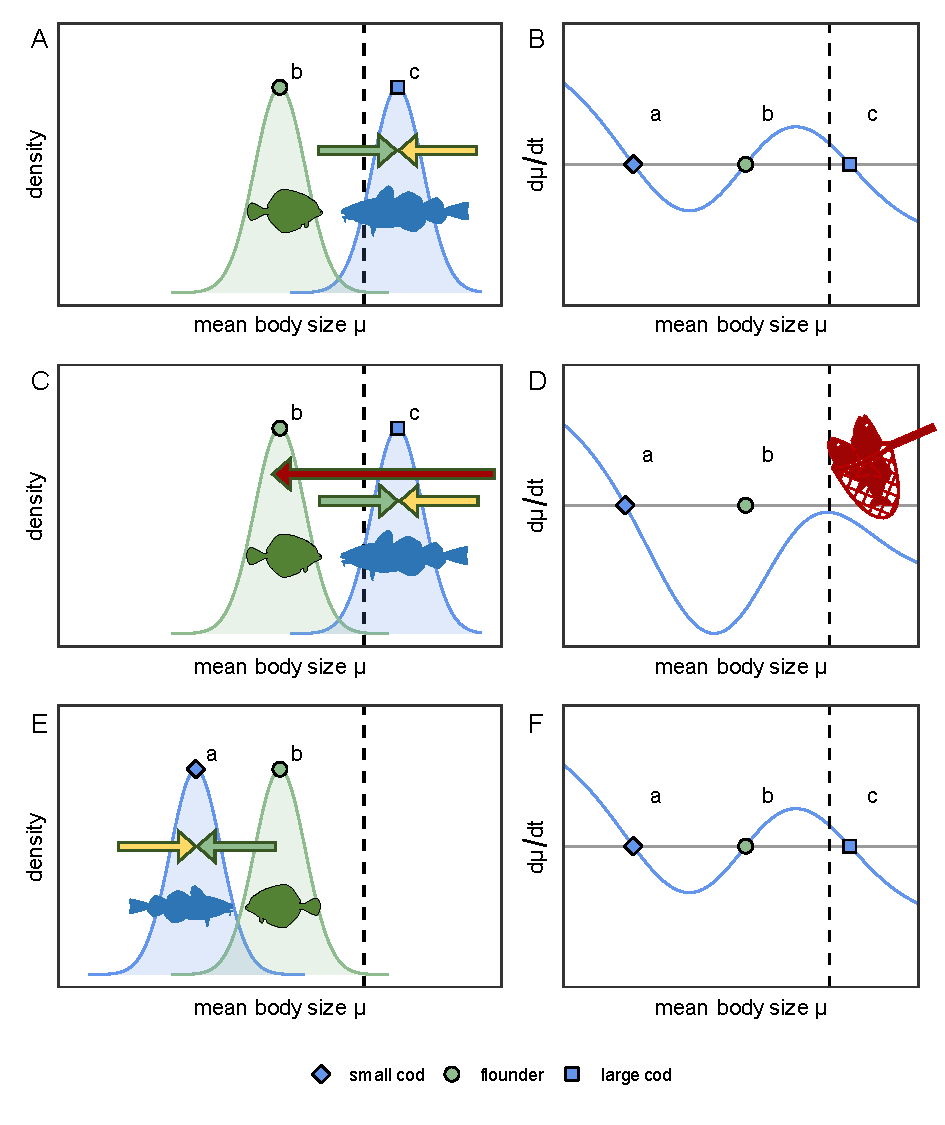
\includegraphics[width=0.9\linewidth]{fig1.pdf}
\caption{}
\label{fig:sizegrid}
\end{figure}

\clearpage

\begin{figure}[!ht]
\centering
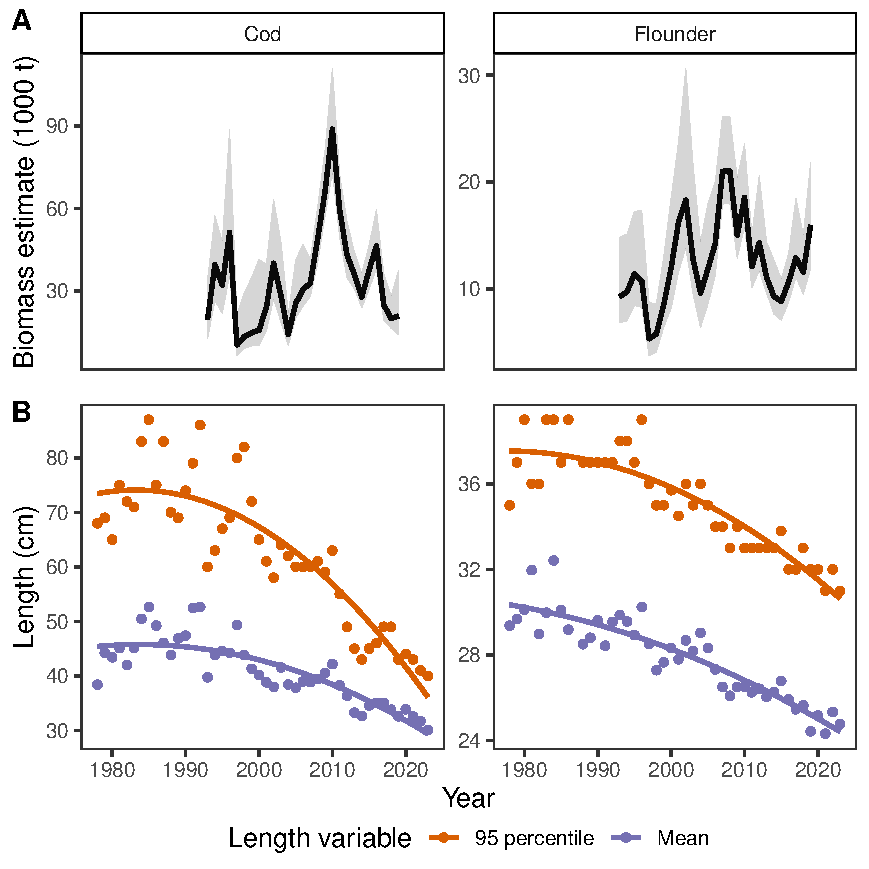
\includegraphics[width=0.8\linewidth]{size_biomass.pdf}
\caption{}
\label{fig:biomasslength}
\end{figure}

\clearpage

\begin{figure}[!ht]
\centering
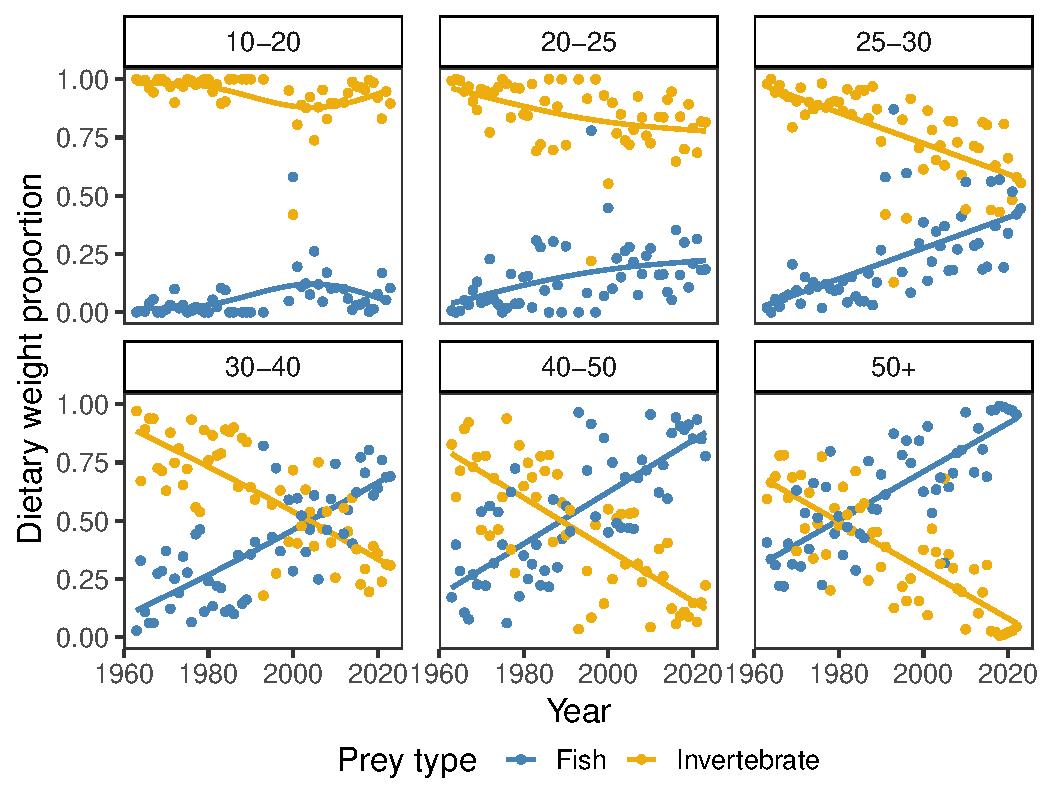
\includegraphics[width=0.8\linewidth]{diet_transition_v2.pdf}
\caption{}
\label{fig:diet_prop}
\end{figure}

\clearpage

\begin{figure}[!ht]
\centering
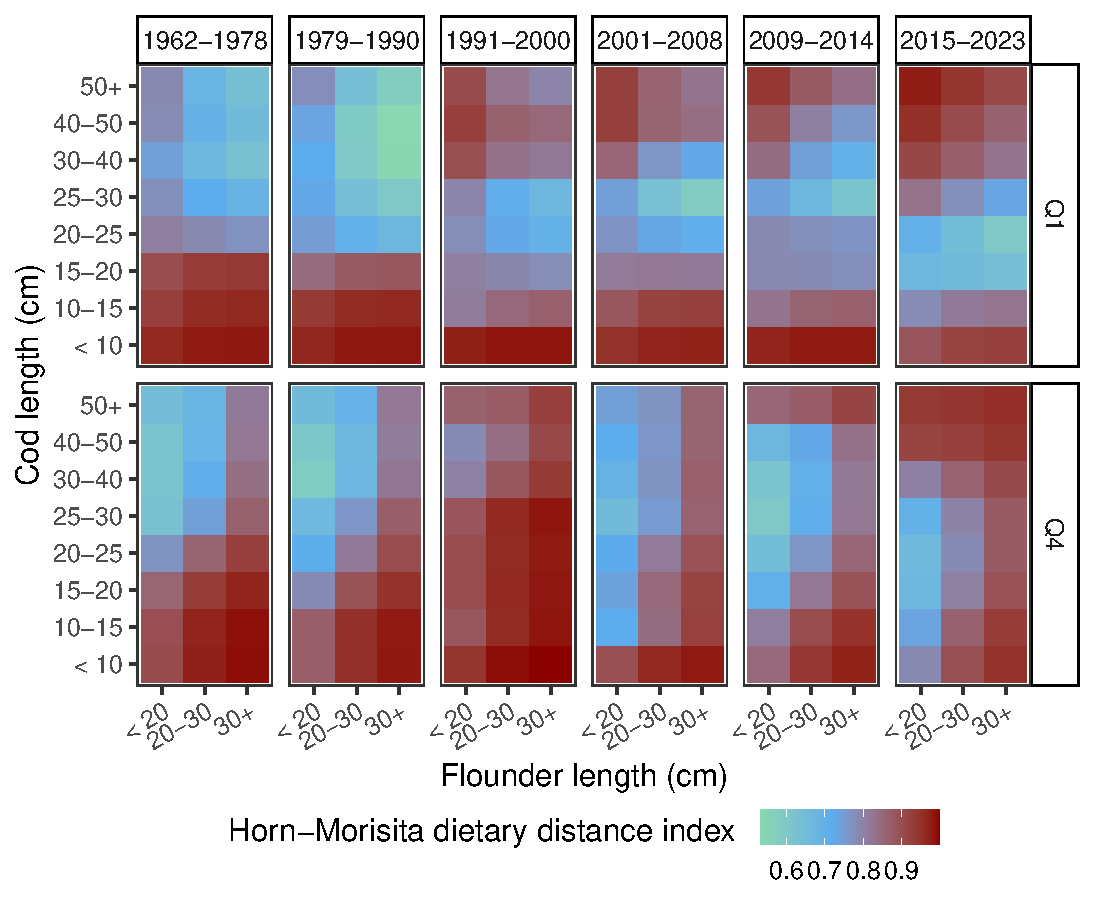
\includegraphics[width=1\linewidth]{diet_mori_v2.pdf}
\caption{}
\label{fig:diet_dist}
\end{figure}

% Figure captions
\subsection*{Figure captions}
{\bf Figure 1:} Conceptual figure of the model exemplified with cod and flounder. Panels A,C,E: cod (blue) and flounder (green) relative body size distributions. Interspecific competition is assumed to increase as the difference between the body size distributions decreases. Arrows represent different sources of selection on cod: green is the selective pressure from flounder competition, yellow from environmental effects, and red from fishing. The dashed lines show the cod's ``optimal'' body size which it would evolve to without competition and fishing. Panels B, D, F: Rate of change of cod mean body size as a function of cod mean body size. Positive (negative) values of $\text{d}\mu/dt$ increase (decrease) cod mean body size. For example in panel B, when mean body size is smaller than $a$, body size increases, while between points $a$ and $b$ body size decreases, making point $a$ a stable equilibrium. Correspondingly, point $c$ is an alternative stable state when cod body size starts larger than $b$. In panel D the rightmost two equilibria are absent (point $b$ is still shown for reference) due to the presence of active fishing which disproportionately selects large cod, overpowering the counterposing pressure from flounder competition.

{\bf Figure 2:} Panel A shows relative annual biomass estimates in 1000 tonnes of cod and flounder in the Baltic Sea over the years 1993--2019. Panel B shows mean and 95th percentile of cod and flounder body length for the years 1978--2023.

{\bf Figure 3:} Cod mean proportional benthic and piscivorous diet, based on stomach content weight for the years 1967--2023 in the Baltic Sea. Facets indicate cod size classes by length (cm).

{\bf Figure 4:} Dietary distance between cod and flounder of different length classes (cm) using the Horn--Morisita index, where 0 indicates identical diet and 1 indicates no similarity. Data based on individual stomach content weight ratios from cod during 1963--2023 and from flounder during 2015--2022, separated into quarters 1 and 4.

\end{document}

